% \chapter{Instandhaltung und Support}

\section{Phase in Softwareprojekten}

	\begin{wrapfigure}[14]{r}{0.45\linewidth}
		\centering
		\vspace{-\baselineskip}
		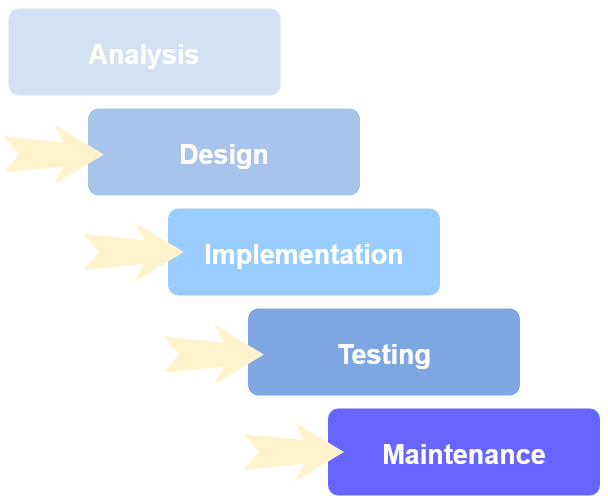
\includegraphics[width=\linewidth]{img/02_maintenance/software-life-cycle.png}
		\caption{Lebenszyklus einer Software}
		\label{fig:software-development-life-cycle}
		\source{Eigene Darstellung von \cite{ASimulationModelWaterfallSoftware}}
	\end{wrapfigure}
	
	In vielen Modellen über den Lebenszyklus einer Software gibt es eine Phase, in der Instandhaltung und Support den Alltag bestimmen, sie wird oftmals ``Maintenance`` bezeichnet \cite{ManagingTheComplexityOfWebSystemsDevelopment} \cite{ASimulationModelWaterfallSoftware}. Sie ist nach Zelkowitz \etal \cite{PrinciplesOfSoftwareEngineeringAndDesign} für rund zwei Drittel der Entwicklungskosten verantwortlich, begründet durch exponentielle Steigung \cite{ExtremeProgrammingExplained}.
	
	Es werden immer bessere Methoden entwickelt, um Probleme in Software - oder auch Bugs - zu verringern. Jedoch erhöht sich zugleich die Komplexität von Software, was zur Ursache hat, dass es mehr Nährboden für Bugs gibt \cite{TrackingDownSoftwareBugsAnomalyDetection}. De-facto sind Bugs ein unvermeidbarer Bestandteil einer Software und müssen daher erwartet und gehandhabt werden \cite{TheMythicalManMonth}.
	
	Wenn nun ein Bug auffällt, sei es durch einen Nutzer oder auch zufällig einem Stakeholder, muss entschieden werden, ob dieser zu beheben ist. Wenn eine Behebung angestrebt wird, benötigt der Stakeholder meistens Rahmeninformationen \cite{WhatMakesAGoodBugReport} um den Bug ggf. zu reproduzieren und die Situation nachzuvollziehen. Desto mehr Verständnis der Stakeholder über das Problem erhält, desto schneller und präziser kann er die Ursache aufdecken. Die Ermöglichung der schnellen Verständnis über ein Problem, wird in dieser Arbeit \textbf{Nachvollziehbarkeit} genannt.

\section{Nachvollziehbarkeit}

	\textit{Hier soll die Nachvollziehbarkeit allgemein beschrieben werden und warum sie erstrebenswert ist.}

	Sie beschäftigt sich mit der Informationserfassung und -aufbereitung, um das Verhalten eines Systems und die Interaktionen der Nutzer für die Stakeholder verständlich zu machen. Sie ist getrennt von der Anstrebung einer Reproduzierbarkeit nach der wissenschaftlichen Methode anzusehen.
	
	{\color{red}\textit{\lipsum[1]}}
	
	Tritt ein Problem bei einem Nutzer auf, aber die Stakeholder erhalten nicht ausreichende Informationen, so kann der Bug ignoriert werden oder in Vergessenheit geraten. Dies geschah im Jahr 2013, als Khalil Shreateh eine Sicherheitslücke bei Facebook fand und bei Facebooks Bug-Bounty-Projekt Whitehat meldete \cite{FacebookBugBounyHunt}. Sein Fehlerreport wurde aufgrund mangelnder Informationen abgelehnt:
	
	\begin{quotation}
	Unfortunately your report [...] did not have enough technical information for us to take action  on  it. We  cannot  respond  to  reports  which  do  not contain enough detail to allow us to reproduce an issue.
	\end{quotation}

\section{Maintenance bei Webapplikationen}

	\textit{Hier sollen die Besonderen Hürden bei Webapplikationen hervorgehoben werden (ungeschulte Nutzer, indirekte Kommunikation, etc.)}
	
	Webapplikationen haben in der Phase der Maintenance ein höheres Potenzial Hindernissen zu begegnen. Einerseits  ist JavaScript dafür bekannt, dass fehleranfälliger Quellcode häufiger auftritt \cite{BuildingStableWebApplications} \cite{BugsJSABenchmarkOfJavaScriptBugs}. Andererseits ist oftmals eine große und breit verteilte Nutzerschaft die Zielgruppe. Dies bedeutet potenziell viele unterschiedliche Umgebungen, stark abweichende Verständnisse einer Webapplikation und indirekte Kommunikationswege zu den Stakeholdern.